\documentclass[12pt]{beamer}

\setbeamertemplate{sidebar right}{}% or get rid of navigation entries there somehow
\addtobeamertemplate{footline}{\hfill\usebeamertemplate***{navigation symbols}%
	\hspace*{0.1cm}\par\vskip 2pt}{}

\AtBeginSection[]
{
	\begin{frame}
	\frametitle{Where are we?}
	\tableofcontents[currentsection]
\end{frame}
}

\usetheme{Singapore}

\usepackage[utf8]{inputenc}
\usepackage{menukeys}
\usepackage{tabularx}
\usepackage{minted}
\usepackage{makecell}
\setminted[bash]{fontsize=\small, tabsize=2, breaklines, linenos}
\setminted[HTML]{fontsize=\small, tabsize=2, breaklines, linenos}

\usepackage[T1]{fontenc}
\usepackage{lmodern}

\graphicspath{ {./images/} }

\title{ 
\includegraphics[width=0.5\linewidth]{hackerschool} \\ Introduction  to Git}
\subtitle{Time to Git Gud}
\author{Raynold Ng Yi Chong}
\date{8 September 2018}

\begin{document}

\frame{\titlepage}

\section{Introduction}
\subsection{}

\begin{frame}
\frametitle{NUS Hackers}

\begin{center}	

\includegraphics[width=0.5\linewidth]{NUSHackers}

\url{http://nushackers.org}
\end{center}

\begin{center}
	\textbf{Hacker}school
	
	Friday \textbf{Hacks}
	
	\textbf{Hack} \& Roll
	
	NUS \textbf{Hacker}space
\end{center}

\end{frame}

\begin{frame}
\frametitle{About Me}

Hi! I am Raynold. My github is \url{https://github.com/raynoldng}

A Year 3 Computer Science Undergraduate who loves building stuff.\\

Have been doing web development for the past 2 years. Interests: algorithms and math

\end{frame}

\begin{frame}
\frametitle{About This Workshop}
\begin{itemize}
	\item Beginner level workshop
	\item No prior knowledge assumed
	\item Basic and advanced features of Git
	\item Better manage your code base and collaborate with others
\end{itemize}
\end{frame}

\begin{frame}
\frametitle{Table of Contents}
\tableofcontents
\end{frame}

\begin{frame}
\frametitle{Required Software}
\begin{itemize}
	\item \textbf{git} (\url{https://git-scm.com/downloads})
	\item \textbf{VS Code} (\url{https://code.visualstudio.com/}) or your favorite text editor
\end{itemize}
\end{frame}


\subsection{Version Control and Git}
\begin{frame}
\frametitle{Have you ever seen:}
\begin{center}	
	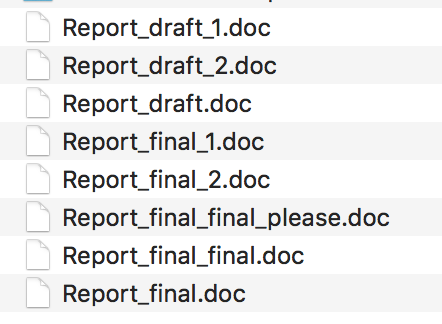
\includegraphics[width=0.5\linewidth]{bad_example}
\end{center}
\end{frame}

\begin{frame}
\frametitle{What is version control}
\begin{itemize}
	\item Category of software tools that help software team manage checks changes to source code over time
	\item every modification to code tracked in a special kind of database
	\item version control software (VSC) essential part of modern software team's professional practices
	\item Example: \url{https://github.com/torvalds/linux/commits/master}
\end{itemize}

\begin{columns}
	\begin{column}{0.33\linewidth}
		
\includegraphics[width=0.8\linewidth]{git_logo}
	\end{column}
	\begin{column}{0.33\linewidth}
		
\includegraphics[width=0.8\linewidth]{mercurial_logo}
	\end{column}
	\begin{column}{0.33\linewidth}
		
\includegraphics[width=0.8\linewidth]{subversion_Logo}
	\end{column}
\end{columns}
\end{frame}

\begin{frame}
\frametitle{What is git?}
\begin{itemize}
	\item Most widely used modern VSC
	\item Originally developed in 2005 by Linus Torvalds, famous creator of Linux operating system kernel
	\item Pros: Performance, Security, Flexibility
	\item Cons: Hard to learn???
	\item Download it here: \url{https://git-scm.com/downloads}
\end{itemize}
\begin{center}	
	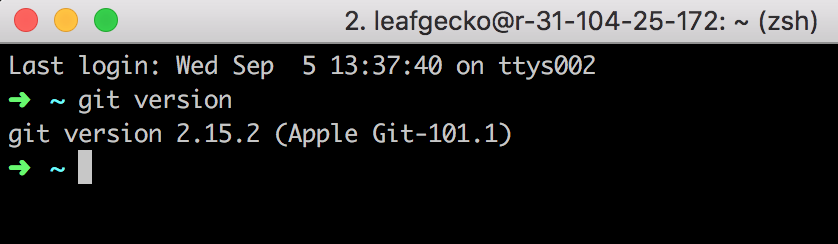
\includegraphics[width=0.5\linewidth]{git_screenshot}
\end{center}
\end{frame}

\begin{frame}[fragile]
\frametitle{Setting up git}
Set your user name and email. Every git commit uses this information and baked into your commits. \mintinline{bash}{--global} option so that git will always use that information on that system
\begin{minted}{bash}
git config --global user.name <your name>
git config --global user.email <your email address>
git config -- global --add color.ui true
\end{minted}
\end{frame}

\section{Getting Started}
\subsection{Setting up a repo}
\begin{frame}[fragile]
\frametitle{Create a local git repo}
\begin{itemize}
	\item When creating a new project on your local machine, you'll first create a new repository
	\item Enter the following into the terminal
\end{itemize}
\begin{center}
\begin{minipage}{0.5\textwidth}
	\begin{minted}{bash}
	cd ~/Desktop
	mkdir my_site
	cd my_site
	git init
	\end{minted}
\end{minipage}
\end{center}
\end{frame}

\begin{frame}
\frametitle{Add a new file to the repo}
\begin{itemize}
	\item We are going to reuse the website created from last week. If you don't have it, get it \href{https://pastebin.com/raw/32W4Ct7k}{here}
	\item once you've added or modified files, in the repo folder, git will notice changes made in the repo
	\item use the \mintinline{bash}{git status} to see which files git knows exist
\end{itemize}
\begin{center}
	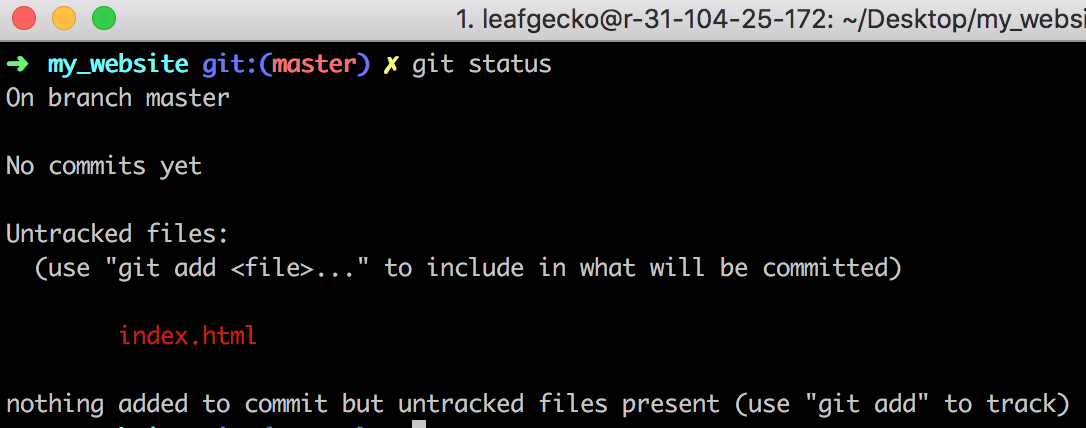
\includegraphics[width=0.5\linewidth]{git_status}
\end{center}
\end{frame}

\subsection{How does git work}
\begin{frame}{Git Basics}
\begin{itemize}
	\item git all about snapshots, not deltas
	\item git thinks of its data as a series of snapshots of a miniature filesystem
	\item every time you commit, git takes a photo of what your files look like and stores a reference to that object
	\item git data is a stream of snapshots 
\end{itemize}
\begin{center}
	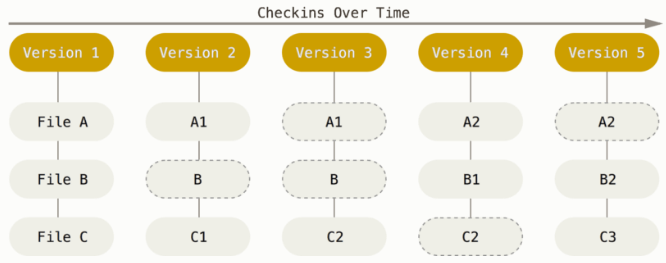
\includegraphics[width=0.7\linewidth]{git_theory}
\end{center}
\end{frame}
\begin{frame}
\frametitle{Master the Three States (Elements)}
\begin{itemize}
	\item \textbf{commit}: record of what files you have changed since the last commit
	\item files in your git repository can be in three main states:
	\begin{itemize}
		\item \textbf{untracked}: any files that are not in your last snap shot and not in your staging area
		\item \textbf{unmodified}: files not modified since last snap shot
		\item \textbf{committed}: data is stored safely in your local database
		\item \textbf{modified}: file changed but have not committed to your database yet
		\item \textbf{staged}: modified file marked in its current version to go into next commit snapshot 
	\end{itemize}
\end{itemize}
\end{frame}

\begin{frame}
\frametitle{git workflow}
\begin{columns}
	\begin{column}{0.5\linewidth}
		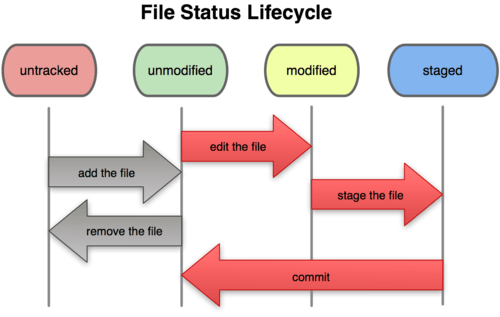
\includegraphics[width=\linewidth]{file_workflow}
	\end{column}
	\begin{column}{0.5\linewidth}
		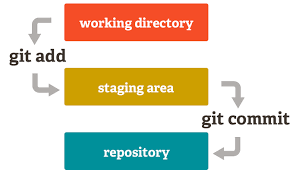
\includegraphics[width=\linewidth]{git_workflow}
	\end{column}
\end{columns}
\end{frame}

\subsection{Saving Changes}
\begin{frame}
\frametitle{Add a file to staging environment}

\begin{itemize}
	\item add a file to staging with the \mintinline{bash}{git add <file>} command
	\item the after \mintinline{bash}{git add}, the file has \textbf{not} yet been added to a commit
\end{itemize}
\begin{center}
	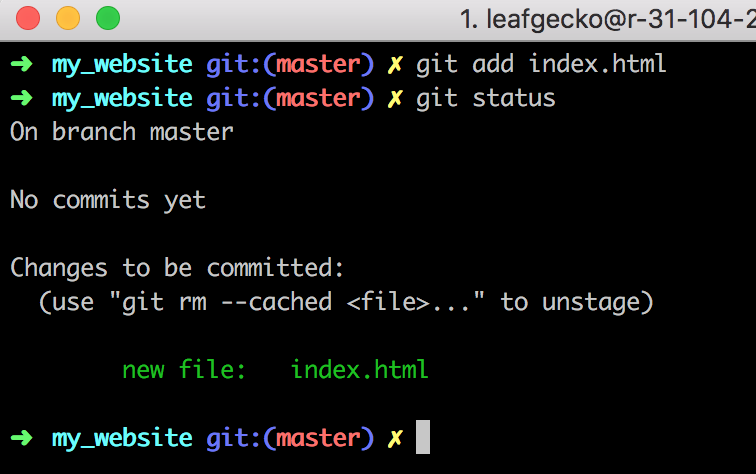
\includegraphics[width=0.7\linewidth]{git_add_screenshot}
\end{center}
\end{frame}

\begin{frame}
\frametitle{Create a commit}
\begin{itemize}
	\item Run the command \mintinline{bash}{git commit -m "Your message to commit"}
	\item The message should be related to the commit
\end{itemize}
\begin{center}
	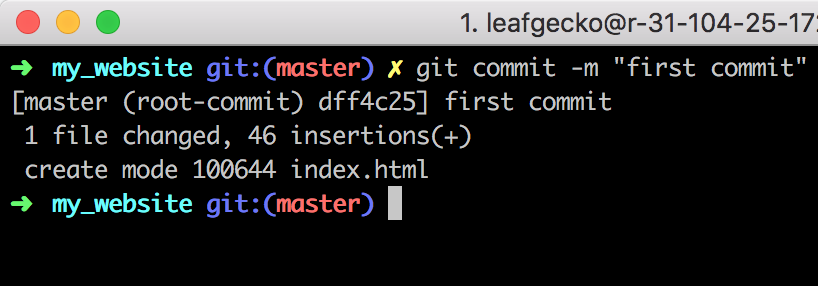
\includegraphics[width=0.7\linewidth]{git_commit_screenshot}
\end{center}
\end{frame}

\begin{frame}
\frametitle{Comparing changes with git diff}
\begin{columns}
	\begin{column}{0.5\linewidth}
		\footnotesize
		\begin{itemize}
			\item Diffing is a function that takes two input data sets and outputs changes between them
			\item Add/delete/edit some lines in \texttt{index.html} and run \mintinline{bash}{git diff} to show any uncommited since last commit
			\item \mintinline{bash}{git diff} used to show changes between commits, commit and working tree etc. See \url{https://git-scm.com/docs/git-diff}{documentation}
		\end{itemize}		
	\end{column}
	\begin{column}{0.5\linewidth}
		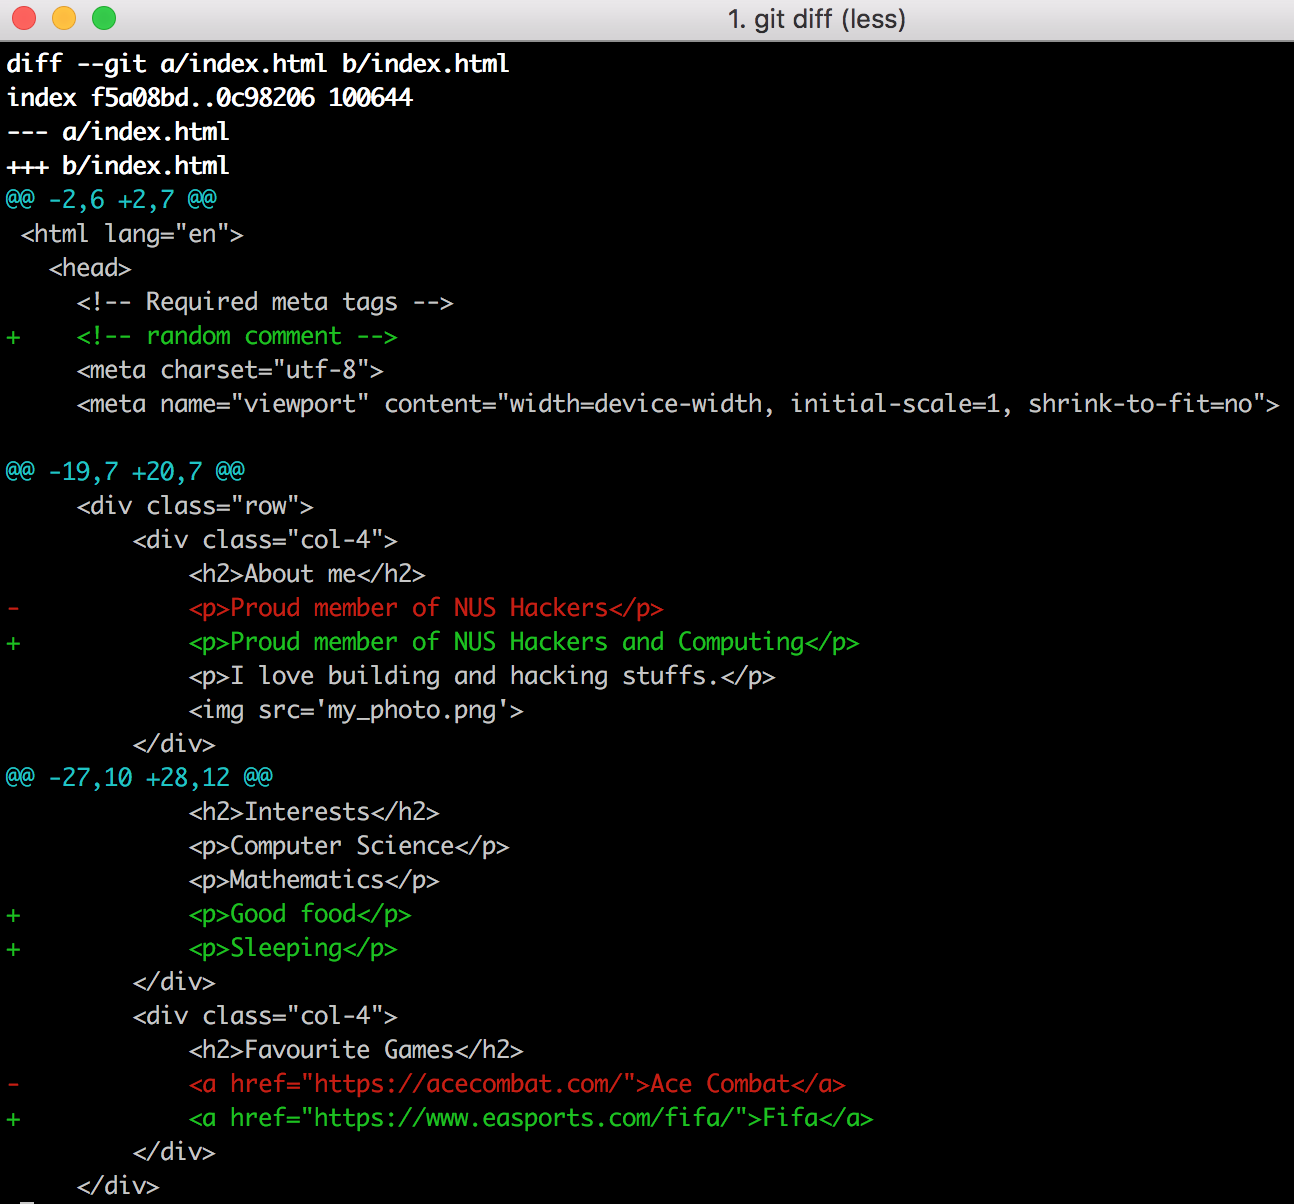
\includegraphics[width=\linewidth]{git_diff_screenshot}
	\end{column}
\end{columns}
\end{frame}

\begin{frame}
\frametitle{Stashing changes}
\begin{itemize}
	\item stashing is handy if you need to quickly switch context and work on something else
	\item \mintinline{bash}{git stash} takes your uncommitted changes (both staged and unstaged) and saves them away for later use
	\item By default, \mintinline{bash}{git stash} will not stash new files and files that are ignored(!), add \mintinline{bash}{-u} or \mintinline{bash}{--include-untracked} to stash untracked files
\end{itemize}
\begin{columns}
	\begin{column}{0.5\linewidth}
		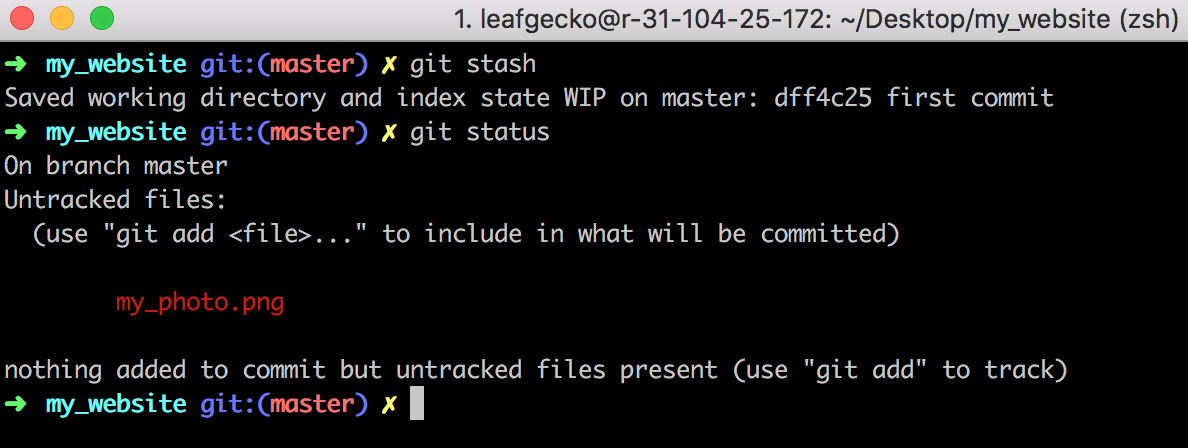
\includegraphics[width=\linewidth]{stash}
	\end{column}
	\begin{column}{0.5\linewidth}
		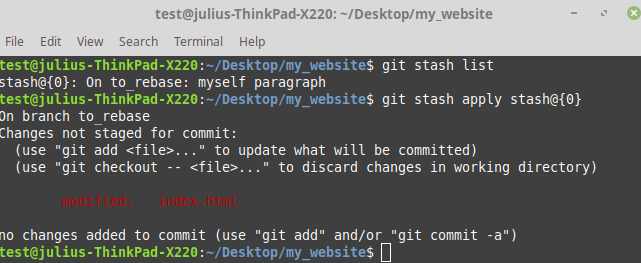
\includegraphics[width=\linewidth]{after_stash}
	\end{column}
\end{columns}
\end{frame}

\begin{frame}
\frametitle{Stashing untracked or ignored files}
\begin{itemize}
	\item By default, \mintinline{bash}{git stash} will not stash new files and files that are ignored(!), add \mintinline{bash}{-u} or \mintinline{bash}{--include-untracked} to stash untracked files
	\item annotate your stash with a description: \mintinline{bash}{git stash save "message"}
\end{itemize}
\begin{center}
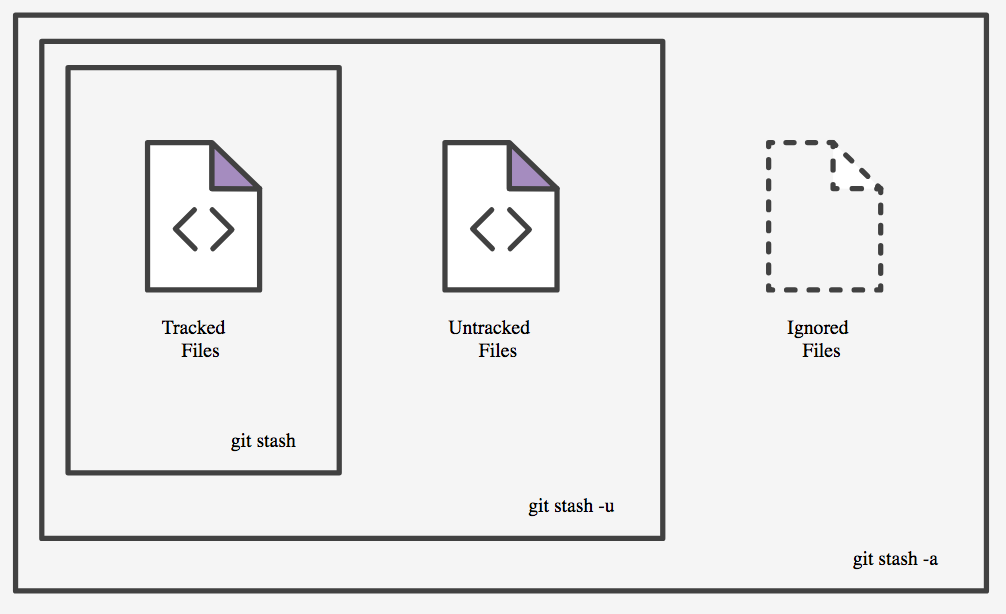
\includegraphics[width=0.5\linewidth]{stash_options}
\end{center}
\end{frame}

\begin{frame}
\frametitle{Applying Stash}
\begin{itemize}
	\item Reapply stashed changes with \mintinline{bash}{git stash pop}
	\item popping \textbf{removes} the changes from your stash and reapplies them to your working copy
	\item \mintinline{bash}{git stash apply} to reapply changes to your working copy and keep them, useful if want to apply on multiple branches(!)
\end{itemize}
\end{frame}

\begin{frame}
\frametitle{.gitignore}
\begin{itemize}
	\item Ignored files are usually build artifacts and machine generated files that can be derived from your repository 
	\item common examples:
	\begin{itemize}
		\item dependency caches like \texttt{/node\_modules} or \text{/packages} 
		\item compiled code, such as .o, .pyc, and .class files
		\item build output directories, such as /bin, /out, or /target
		\item files generated at runtime, such as .log, .lock, or .tmp
		\item personal config files like \texttt{.idea/workspace}
	\end{itemize}
\end{itemize}
\end{frame}

\begin{frame}
\frametitle{Git ignore patterns}
\begin{itemize}
	\item **/logs
	\item **/logs/debug.log
	\item *.log
	\item /debug.log
	\item debug.log
	\item See the full list \href{https://www.atlassian.com/git/tutorials/saving-changes/gitignore}{here}
\end{itemize}
\end{frame}

\section{Collaborating}
\subsection{Branching}
\begin{frame}
\frametitle{Branching}
\begin{itemize}
	\item allow you to diverge from the main line of development and continue work without messing with the main line	
	\item killer feature of git as it is incredibly fast and lightweight
	\item a branch is a lightweight pointer to a commit, default pointer is \texttt{master}
	\item \texttt{HEAD}: special pointer to local branch that you are currently on
\end{itemize}
\begin{center}
	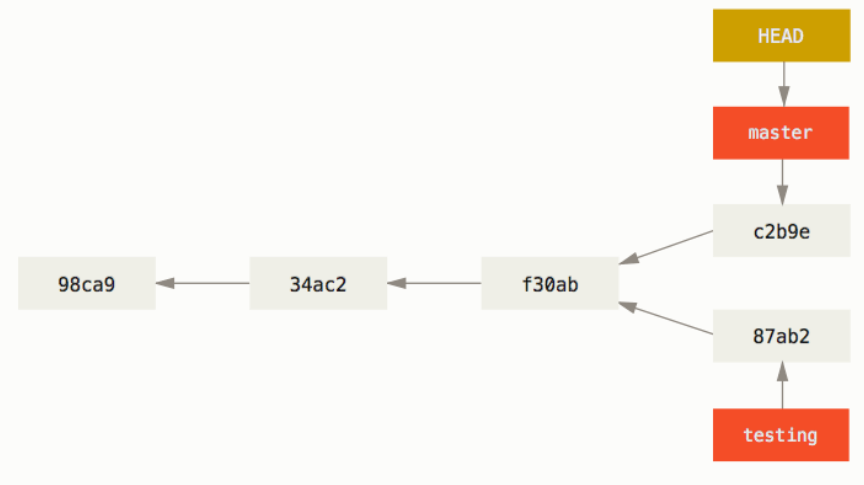
\includegraphics[width=0.7\linewidth]{branching}
\end{center}
\end{frame}

\begin{frame}
\frametitle{Common branch commands}
\begin{itemize}
	\item \mintinline{bash}{git branch}: list all branches
	\item \mintinline{bash}{git branch <branch>}: create a new branch of given name
	\item \mintinline{bash}{git branch -d <branch>}: delete specified branch, cannot delete if have unmerged changes
	\item \mintinline{bash}{git branch -D <branch>}: force delete specified branch
	\item \mintinline{bash}{git branch -m <branch>}: rename current branch to <branch>
	\item \mintinline{bash}{git branch -a}: list all remote branches
\end{itemize}
\end{frame}

\begin{frame}
\frametitle{Git checkout}
\begin{center}
	
\includegraphics[width=0.6\linewidth]{checkout_meme}
\end{center}
\end{frame}

\begin{frame}[fragile]
\frametitle{Creating and checking out a branch}
\begin{itemize}
	\item checking out is the act of switching between different versions of a target entity
	\item entities: files, commits, and branches
\end{itemize}
\begin{minted}{bash}
git branch personal_photo
git checkout personal_photo
\end{minted}
OR:
\begin{minted}{bash}
git checkout -b personal_photo
\end{minted}
\begin{center}
	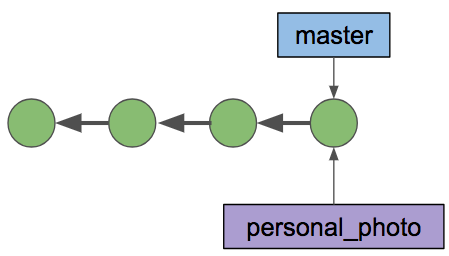
\includegraphics[width=0.55\linewidth]{branch_diagram}
\end{center}
\end{frame}

\begin{frame}
\frametitle{Branching Workflow}
\begin{enumerate}
	\item add photo to \texttt{index.html} and commit it, doing so moves \texttt{personal\_photo} forward
	\item urgent fix: change the name, create a \texttt{hot\_fix} branch, once done merge it back into \texttt{master}
	\item switch back to adding your photo and merge it back into master when done
\end{enumerate}
\begin{columns}
	\begin{column}{0.33\linewidth}
		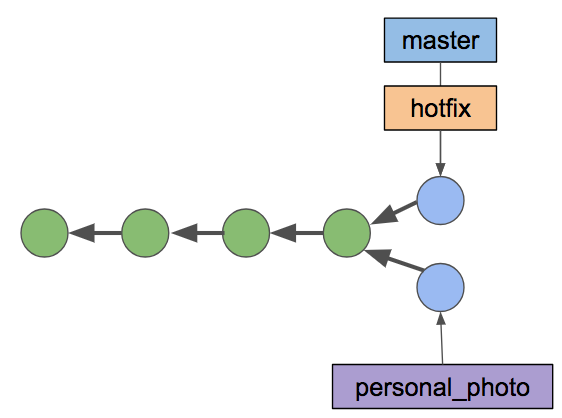
\includegraphics[width=\linewidth]{branch_1}
	\end{column}
	\begin{column}{0.33\linewidth}
		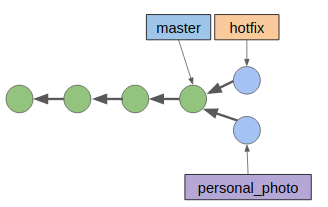
\includegraphics[width=\linewidth]{branch_2}
	\end{column}
	\begin{column}{0.33\linewidth}
		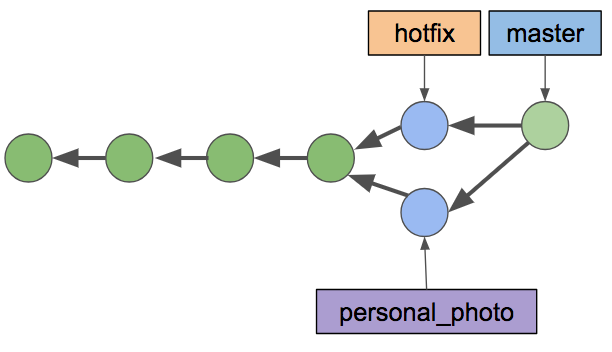
\includegraphics[width=\linewidth]{branch_3}
	\end{column}
\end{columns}
\end{frame}

\begin{frame}{git fast forwarding}
\begin{itemize}
	\item git does a fast forward when you merge a branch that is ahead of your checked out branch (e.g. merge \texttt{hotfix} into \texttt{master}
	\item both branches point the same commit and no new commit is made	
\end{itemize}
\begin{center}
	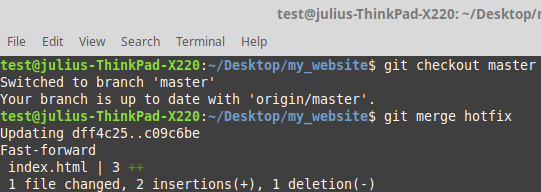
\includegraphics[width=\linewidth]{fast_forward}
\end{center}
\end{frame}

\begin{frame}{Three way merge}
\begin{itemize}
	\item however a three way merge is not possible if branches have diverged
	\item git has to do a 3 way merge, a dedicated commit is used to tie together the two histories
	\item 3 way: three commits to generate the merge commit: two branch tips and their common ancestor
	\item \mintinline{bash}{git log --oneline --decorate --graph --all}
\end{itemize}
\begin{columns}
	\begin{column}{0.5\linewidth}
		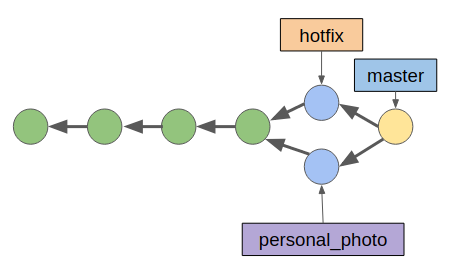
\includegraphics[width=\linewidth]{three_way_merge}
	\end{column}
	\begin{column}{0.5\linewidth}
		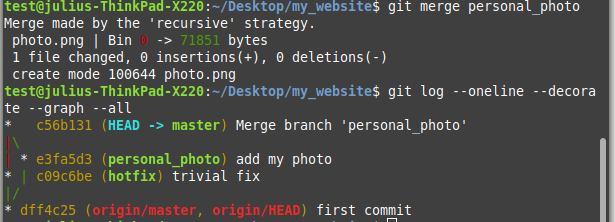
\includegraphics[width=\linewidth]{merge_screenshot}
	\end{column}
\end{columns}
\end{frame}

\subsection{Collabing Online}
\begin{frame}
\frametitle{What is Github?}
\begin{itemize}
	\item code hosting platform for version control and collaboration. It lets you and others work together on projects from anywhere
	\item alternative: bitbucket
\end{itemize}
\begin{center}
	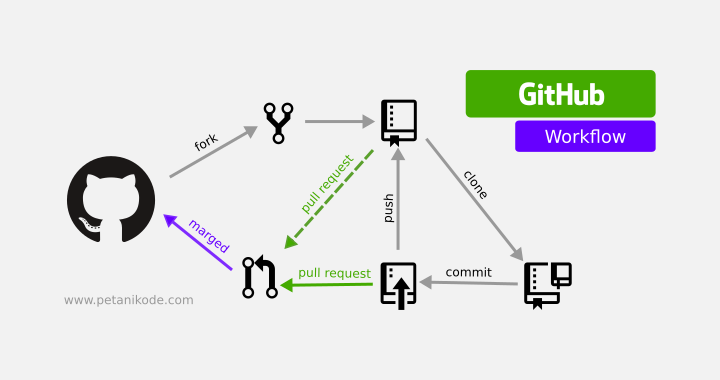
\includegraphics[width=0.75\linewidth]{github-workflow}
\end{center}
\end{frame}

\begin{frame}[fragile]
\frametitle{Create your github repo}
\begin{enumerate}
	\item Create a github account if you haven't done so already
	\item Create a new repository \texttt{my website} or any name you want
	\item Push your code to this repo
\end{enumerate}
\begin{columns}
	\begin{column}{0.5\linewidth}
		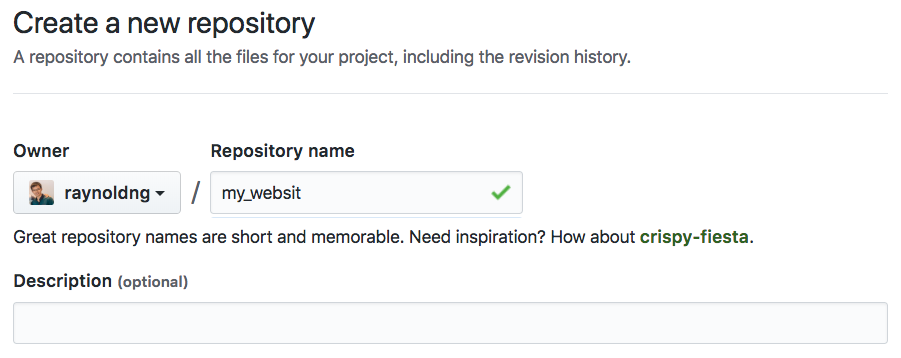
\includegraphics[width=\linewidth]{new_github_repo}
	\end{column}
	\begin{column}{0.5\linewidth}
		\tiny
		\begin{minted}{bash}
		git remote add origin <url>
		git push -u origin master
		\end{minted}
	\end{column}
\end{columns}
\end{frame}

\begin{frame}
\frametitle{Working with remotes}
\begin{itemize}
	\item remote repos are versions of your project that are hosted on the Internet (Github) or somewhere
	\item collaborating with others involves managing these remote repositories and pushing and pulling data between them
\end{itemize}
\begin{center}
	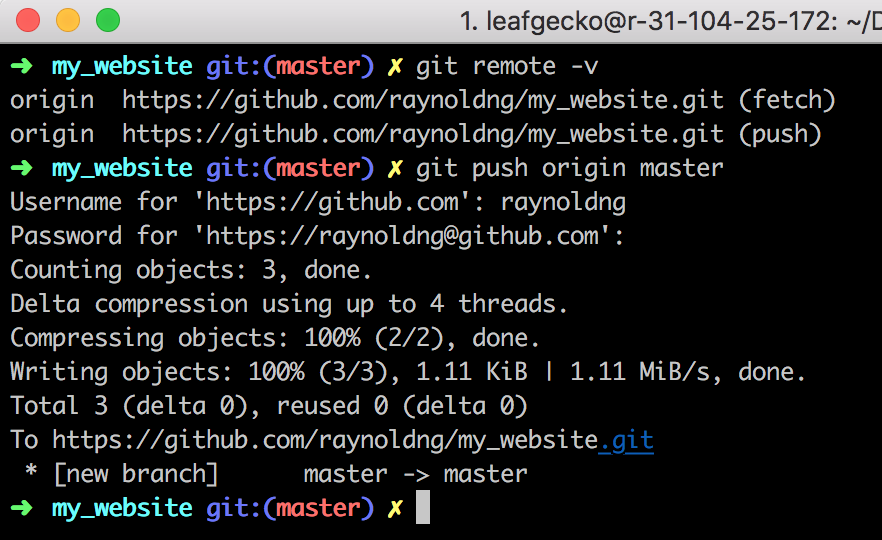
\includegraphics[width=0.8\linewidth]{git_remote}
\end{center}
\end{frame}

\begin{frame}
\frametitle{Fetching, Pushing and Pulling}
\begin{itemize}
	\item \mintinline{bash}{git fetch <remote>}: goes to remote project and pulls down all the data from that remote project that you don’t have yet
	\item \mintinline{bash}{git pull <remote>}: fetch and merge that remote branch into your current branch
	\item \mintinline{bash}{git push <remote> <branch>}: push branch to remote project, you need write permissions to that remote project
\end{itemize}
\end{frame}

\begin{frame}
\frametitle{Cloning a repo}
\begin{itemize}
	\item \mintinline{bash}{git clone} target an existing repo and create a clone, or copy of the target repository
	\item cloning automatically creates a remote connection called origin pointing back to the original repository
\end{itemize}
\begin{center}
	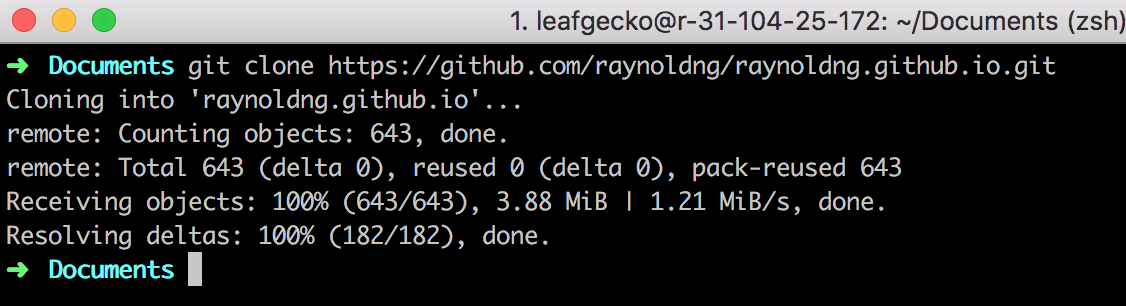
\includegraphics[width=\linewidth]{git_clone}
\end{center}
\end{frame}

\begin{frame}
\frametitle{Forking a repo}
\begin{itemize}
	\item forking produces a personal copy of someone else's project
	\item acts as the bridge between original repository and your personal copy
	\item you can submit pull requests to help make other people's project better
\end{itemize}
\begin{center}
	
\includegraphics[width=0.8\linewidth]{forking}
\end{center}
\end{frame}

\begin{frame}
\frametitle{Making a Pull Request}
\begin{itemize}
	\item mechanism for a developer to notify team members that they have completed a feature
	\item once feature is ready, the dev files a pull request via their Github account
	\item pull request is more than just a notification—it’s a dedicated forum for discussing the proposed feature
\end{itemize}
\begin{center}
	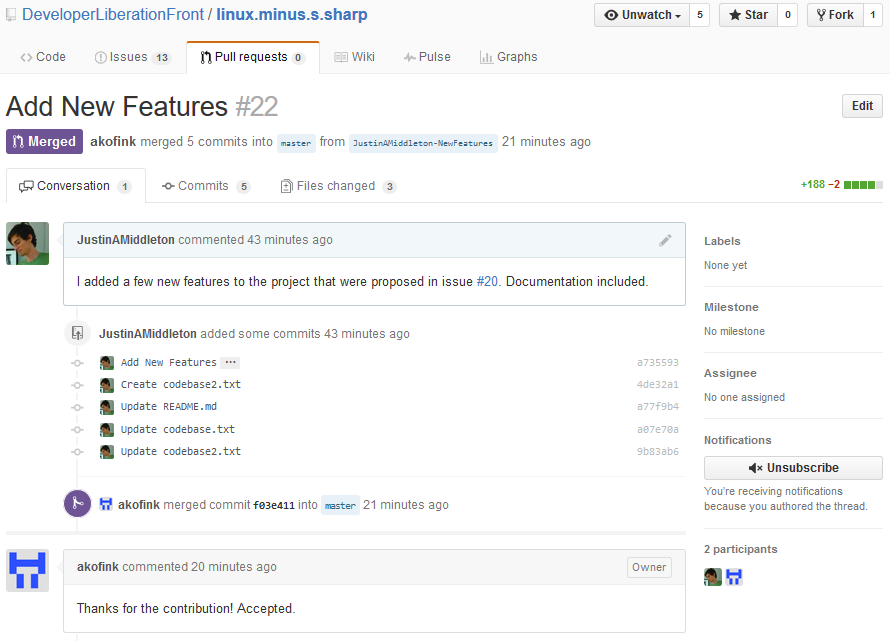
\includegraphics[width=0.8\linewidth]{pull_request_example}
\end{center}
\end{frame}

\begin{frame}
\frametitle{Pair Activity}
\begin{enumerate}
	\item Learn one interesting fact about the person sitting next to you
	\item Fork his/her project and create a branch \texttt{fun\_facts} and add the fun fact under the \texttt{About Me} section
	\item Create a pull request
	\item Accept your neighbor's pull request
\end{enumerate}
\end{frame}

\section{Advanced Features}
\subsection{Rebasing}
\subsection{Reset, Checkout, Revert}
\subsection{Cherry Picking}

\section{Conclusion}
\subsection{Quality of Life Improvements}

\begin{frame}
\frametitle{Talk to us!}
\begin{itemize}
	\item \textbf{Feedback form}: \url{https://tinyurl.com/hs2018-html}
	\item \textbf{Completed:}
	\begin{itemize}
		\item HTML/CSS
		\item Git
	\end{itemize}
	\item \textbf{Upcoming hackerschool}:
	\begin{itemize}
		\item HTML/CSS practice
		\item Introduction to ES6
	\end{itemize}
\end{itemize}
\end{frame}


\end{document}